\documentclass[11pt]{article}

\usepackage[margin=1in]{geometry}
\usepackage{amsmath,amssymb,mathtools}
\usepackage{booktabs}
\usepackage{graphicx}
\usepackage{float}

\setlength{\parindent}{0pt}
\setlength{\parskip}{0.55em}
\renewcommand{\arraystretch}{1.15}

\newcommand{\diag}{\operatorname{diag}}
\newcommand{\norm}[1]{\left\lVert #1\right\rVert}

\title{Problem 4 Handout III\\Chebyshev Collocation for Burgers' Equation on $(-1,1)$}
\author{Rishabh Kumar}
\date{\today}

\begin{document}
\maketitle

\section{Interval Problem}

The final part of Question 4 considers
\begin{equation}
    u_t+u u_x=\varepsilon u_{xx},
    \qquad -1<x<1,\quad t>0,
    \label{eq:burgers}
\end{equation}
with
\begin{equation}
    u(-1,t)=u(1,t)=0,
    \qquad
    u(x,0)=-\sin(\pi x),
    \qquad
    \varepsilon=0.02,
    \qquad
    T=0.995.
    \label{eq:interval-data}
\end{equation}
The conservative form is
\begin{equation}
    u_t+\frac12(u^2)_x=\varepsilon u_{xx}.
    \label{eq:conservative}
\end{equation}

\section{Fourier Versus Chebyshev Collocation}

Fourier collocation is natural on periodic domains, because the basis functions
$e^{ikx}$ automatically satisfy periodicity.  The interval problem \eqref{eq:interval-data}
is not periodic: it has Dirichlet boundary conditions at $x=\pm1$.  The standard
spectral collocation replacement is therefore Chebyshev collocation.

Chebyshev collocation uses algebraic polynomials instead of trigonometric
polynomials.  Its collocation nodes cluster near the endpoints, which is useful for
viscous Burgers' equation because steep gradients and boundary layers can form near
$x=\pm1$.

\section{Chebyshev--Lobatto Nodes}

For polynomial degree $N$, define the Chebyshev--Lobatto points
\begin{equation}
    x_j=\cos\left(\frac{j\pi}{N}\right),
    \qquad
    j=0,1,\ldots,N.
    \label{eq:lobatto}
\end{equation}
These points include both endpoints:
\begin{equation}
    x_0=1,
    \qquad
    x_N=-1.
\end{equation}
The points are not uniformly spaced.  They are dense near $x=\pm1$ and relatively
coarse near the centre.

\begin{figure}[H]
    \centering
    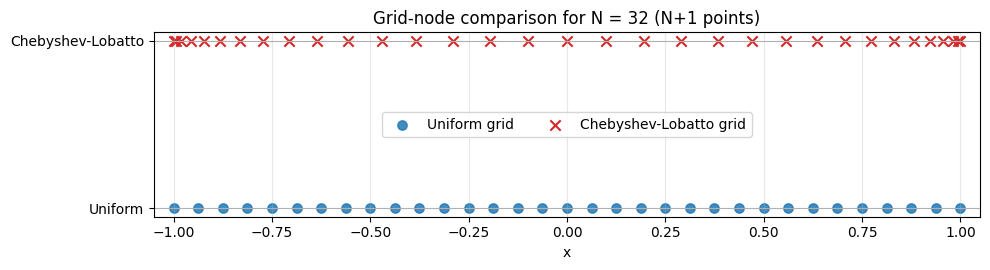
\includegraphics[width=0.88\textwidth]{figures/grid_comparison.png}
    \caption{Uniform grid versus Chebyshev--Lobatto grid.  The Chebyshev nodes cluster near the endpoints.}
\end{figure}

\section{Differentiation Matrix}

Let $U_j(t)\approx u(x_j,t)$ be the nodal values, and let $p_N(x)$ be the degree $N$
polynomial interpolating these values:
\begin{equation}
    p_N(x_j)=U_j,
    \qquad
    j=0,\ldots,N.
\end{equation}
The derivative of the interpolant at the nodes is represented by a dense matrix
$D$:
\begin{equation}
    p_N'(x_i)\approx \sum_{j=0}^{N}D_{ij}U_j.
\end{equation}
For $i\ne j$,
\begin{equation}
    D_{ij}
    =
    \frac{c_i}{c_j}
    \frac{(-1)^{i+j}}{x_i-x_j},
    \qquad
    c_0=c_N=2,
    \qquad
    c_j=1\quad(1\le j\le N-1).
    \label{eq:D-offdiag}
\end{equation}
The diagonal entries are chosen so that the derivative of a constant is zero:
\begin{equation}
    D_{ii}=-\sum_{j\ne i}D_{ij}.
\end{equation}
Equivalently, one may use the standard explicit diagonal formulas
\begin{equation}
    D_{00}=\frac{2N^2+1}{6},
    \qquad
    D_{NN}=-\frac{2N^2+1}{6},
    \qquad
    D_{ii}=-\frac{x_i}{2(1-x_i^2)}
    \quad(1\le i\le N-1).
\end{equation}
The second derivative matrix is
\begin{equation}
    D^{(2)}=D^2.
\end{equation}
Unlike finite-difference matrices, $D$ and $D^2$ are dense.  This is the price paid
for spectral accuracy.

\section{Semi-Discrete Burgers System}

Using the conservative form \eqref{eq:conservative}, the Chebyshev collocation
semi-discretisation is
\begin{equation}
    \dot U+\frac12D(U\odot U)=\varepsilon D^2U,
    \label{eq:semi}
\end{equation}
where $\odot$ denotes componentwise multiplication:
\begin{equation}
    (U\odot U)_j=U_j^2.
\end{equation}
The boundary conditions are imposed strongly:
\begin{equation}
    U_0(t)=0,
    \qquad
    U_N(t)=0.
\end{equation}
Let
\begin{equation}
    I=\{1,2,\ldots,N-1\}
\end{equation}
denote the interior nodes.  Only the interior nodal values are unknown.

\section{CNLF Time Discretisation}

Applying the same CNLF idea as in the finite-difference method gives
\begin{equation}
    \frac{U^{n+1}-U^{n-1}}{2k}
    +
    \frac12D\bigl((U^n)^2\bigr)
    =
    \frac{\varepsilon}{2}D^2(U^{n+1}+U^{n-1}).
    \label{eq:cheb-cnlf-full}
\end{equation}
Restricting to interior nodes and imposing $U_0^{n+1}=U_N^{n+1}=0$, the unknown
interior vector satisfies
\begin{equation}
    \left(I-\varepsilon kD^2_{II}\right)U_I^{n+1}
    =
    U_I^{n-1}
    +
    \varepsilon k(D^2U^{n-1})_I
    -
    \frac{k}{2}
    \left(D\bigl((U^n)^2\bigr)\right)_I.
    \label{eq:cheb-cnlf}
\end{equation}
This is a linear solve for $U_I^{n+1}$.  The nonlinear term is explicit because it is
evaluated at time level $n$.

\section{Why a Newton Solve Appears in the Startup}

CNLF is a two-step method, so it requires both $U^0$ and $U^1$.  The initial value is
\begin{equation}
    U_j^0=-\sin(\pi x_j).
\end{equation}
The notebook computes $U^1$ using one nonlinear Crank--Nicolson startup step:
\begin{equation}
    U^1-U^0
    +
    \frac{k}{4}D\left((U^1)^2+(U^0)^2\right)
    -
    \frac{\varepsilon k}{2}D^2(U^1+U^0)
    =
    0.
    \label{eq:startup}
\end{equation}
This startup equation treats the nonlinear Burgers flux implicitly through
$(U^1)^2$.  That is why Newton's method is used.  The Chebyshev derivatives themselves
are not computed by Newton; they are supplied by the matrices $D$ and $D^2$.

To write the Newton system, let $W$ denote the unknown interior vector at time $k$,
and let $\widehat W$ be the full vector with boundary values
\begin{equation}
    \widehat W_0=\widehat W_N=0,
    \qquad
    \widehat W_I=W.
\end{equation}
Define the residual on the interior nodes by
\begin{equation}
\begin{aligned}
    F(W)
    &=
    W-U_I^0
    +
    \frac{k}{4}
    \left(D\left(\widehat W\odot \widehat W+U^0\odot U^0\right)\right)_I
    \\
    &\qquad
    -
    \frac{\varepsilon k}{2}
    \left(D^2(\widehat W+U^0)\right)_I.
\end{aligned}
\end{equation}
The Jacobian is
\begin{equation}
    J(W)
    =
    I
    +
    \frac{k}{2}D_{II}\diag(W)
    -
    \frac{\varepsilon k}{2}D^2_{II}.
    \label{eq:newton-jacobian}
\end{equation}
Newton's method updates
\begin{equation}
    J(W^{(\ell)})\,\Delta W^{(\ell)}
    =
    -F(W^{(\ell)}),
    \qquad
    W^{(\ell+1)}=W^{(\ell)}+\Delta W^{(\ell)}.
\end{equation}
After this startup, all later CNLF steps use the linear solve
\eqref{eq:cheb-cnlf}.

\section{Parameters and Numerical Result}

The notebook uses
\begin{equation}
    N=96,
    \qquad
    k=10^{-3},
    \qquad
    \varepsilon=0.02,
    \qquad
    T=0.995.
\end{equation}
The Chebyshev-CNLF solution captures the same steepening and viscous smoothing seen
in the finite-difference reference computation.

\begin{figure}[H]
    \centering
    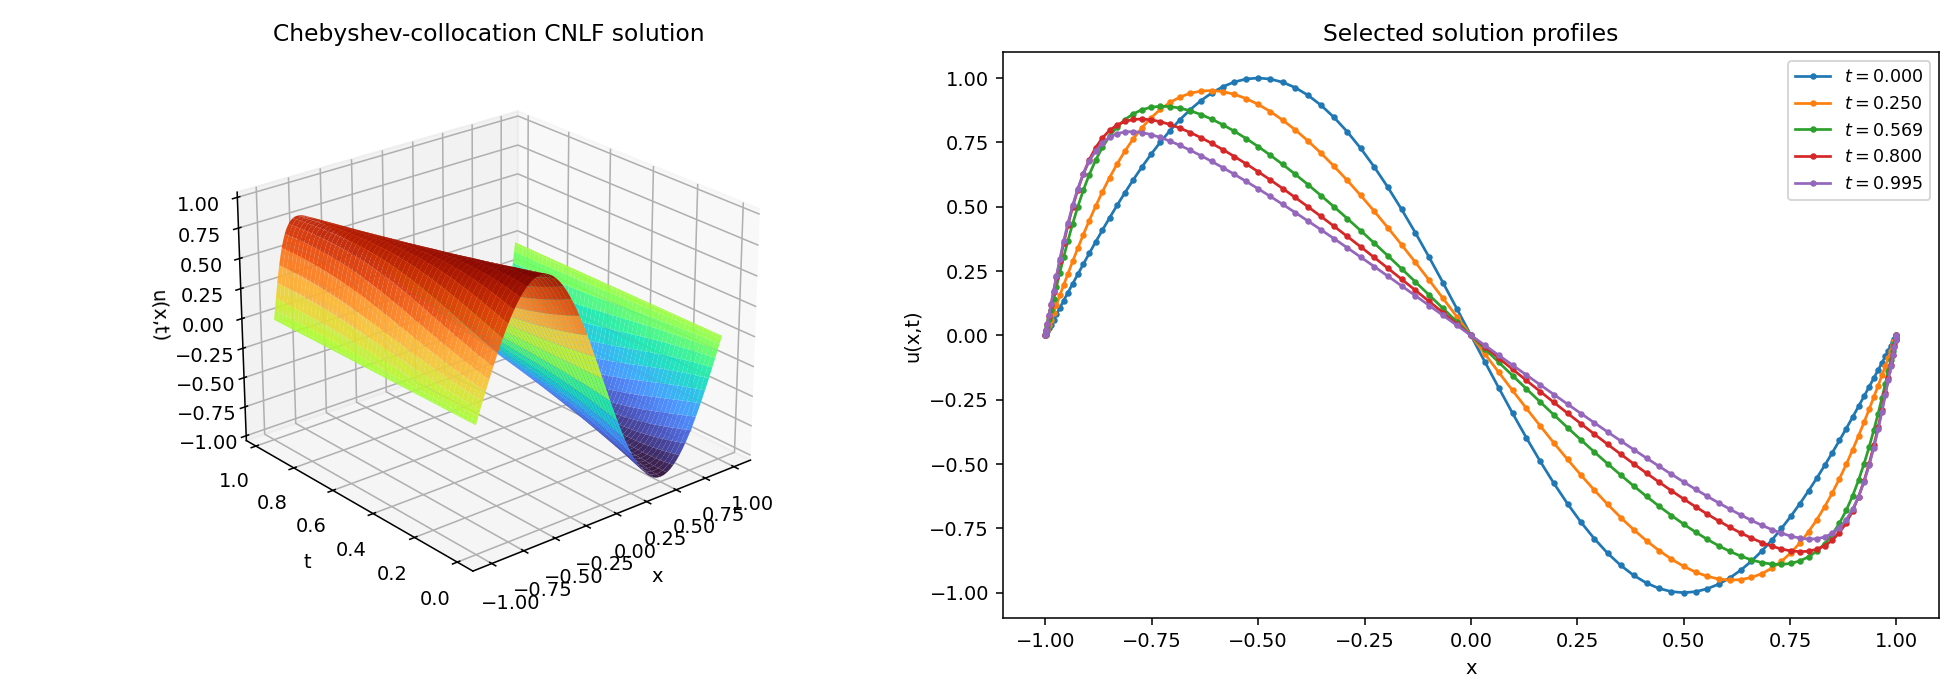
\includegraphics[width=\textwidth]{figures/chebyshev_collocation.png}
    \caption{Chebyshev-collocation CNLF solution and selected profiles.}
\end{figure}

\begin{figure}[H]
    \centering
    
\includegraphics[width=0.78\textwidth]{figures/burgers_sine.png}
    \caption{Finite-difference CNLF reference profiles for the same interval problem.}
\end{figure}

\section{Summary}

The Chebyshev method is the spectral collocation analogue of Fourier collocation for
a nonperiodic interval.  The spatial derivative is represented by dense
differentiation matrices on Chebyshev--Lobatto nodes, while the time discretisation is
the same CNLF idea used in the finite-difference part.  Newton's method is needed only
for the nonlinear Crank--Nicolson startup step; after that, the CNLF update is linear
at each time step.

\end{document}
